\begin{figure}[H]%
		\ThisCenterWallPaper{1}{images/\texorpdfstring{\chaptername\thechapter}}%
		\captionlistentry[figure]{Icon of \chaptername\ \thechapter}% figure with chapter and section number
		%\addcontentsline{lof}{figure}{Icon of \chaptername\ \thechapter}% figure without chapter and section number
		\label{fig:\chaptername\thechapter}%
\end{figure}

\vspace*{-1.45cm}
\noindent \large{\textbf{This {\MakeLowercase{\chaptername}}'s contents:}}
\vspace*{-0.65cm}
\minitoc \mtcskip \minilof
\vspace*{-1.0cm}
\section[GraphQL API Schema]{\gls{GraphQL} \acrshort{API} Schema} \label{section:APIDocs/GraphQLAPISchema}
The \gls{GraphQL schema} is composed of the type definitions shown in \hyperref[code:adomainthatrocksbackend/graphql/schema]{\autoref{code:adomainthatrocksbackend/graphql/schema}}.

\begin{sublstlisting}
    Specifically types are defined for \texttt{Author}: \hyperref[code:adomainthatrocksbackend/graphql/schema12]{\autoref{code:adomainthatrocksbackend/graphql/schema12}}, \texttt{Publication}: \hyperref[code:adomainthatrocksbackend/graphql/schema27]{\autoref{code:adomainthatrocksbackend/graphql/schema27}}, \texttt{Institution}: \hyperref[code:adomainthatrocksbackend/graphql/schema34]{\autoref{code:adomainthatrocksbackend/graphql/schema34}}, \texttt{Community}: \hyperref[code:adomainthatrocksbackend/graphql/schema39]{\autoref{code:adomainthatrocksbackend/graphql/schema39}} and others that are not presented here. For a complete list of type definitions of the \gls{GraphQL schema}, see \hyperref[subsection:SourceCode/Instructionshowtorunbuildanddeploy/Backendssourcecode]{\S\ \ref{subsection:SourceCode/Instructionshowtorunbuildanddeploy/Backendssourcecode}} on \hyperref[subsection:SourceCode/Instructionshowtorunbuildanddeploy/Backendssourcecode]{page \ref*{subsection:SourceCode/Instructionshowtorunbuildanddeploy/Backendssourcecode}}.
    
    \noindent\lstinputlisting[
        %nolol, % will not appear in list of code listings
        linerange = {12-26}, % choose line numbers to include
        firstnumber = 12,
        language = GraphQL,
        mathescape = false,
        label = {code:adomainthatrocksbackend/graphql/schema12},
        caption = {[\ \ \ \ \ \ \ The Author type]The Author type}
    ]{code/adomainthatrocksbackend/graphql/schema.js}
    
    Even though not shown here for brevity, \texttt{Affiliation} and \texttt{Note} types are defined in previous lines of code.
    
    \noindent\begin{minipage}{\linewidth} % Wraps the lstlisting inside a minipage of width \linewidth with no indentation to prevent it from splitting between pages
        \noindent\lstinputlisting[
            %nolol, % will not appear in list of code listings
            linerange = {27-33}, % choose line numbers to include
            firstnumber = 27,
            language = GraphQL,
            mathescape = false,
            label = {code:adomainthatrocksbackend/graphql/schema27},
            caption = {[\ \ \ \ \ \ \ The Publication type]The Publication type}
        ]{code/adomainthatrocksbackend/graphql/schema.js}
    \end{minipage}%
    
    The \texttt{Publication}'s \texttt{author} field is of type \texttt{[String]}.
    This is so because, not all author's attributes are included when asking for a publication, just the names in the form of an array of strings.
    
    \noindent\begin{minipage}{\linewidth} % Wraps the lstlisting inside a minipage of width \linewidth with no indentation to prevent it from splitting between pages
        \noindent\lstinputlisting[
            %nolol, % will not appear in list of code listings
            linerange = {34-38}, % choose line numbers to include
            firstnumber = 34,
            language = GraphQL,
            mathescape = false,
            label = {code:adomainthatrocksbackend/graphql/schema34},
            caption = {[\ \ \ \ \ \ \ The Institution type]The Institution type}
        ]{code/adomainthatrocksbackend/graphql/schema.js}
    \end{minipage}%
    
    All attributes having as value types, types that are followed by an exclamation mark (\texttt{!}), have to be included in the requested fields of a \gls{GraphQL query}.
    The other attributes, whose value types are not followed by an exclamation mark, are optional.
    It is within the developer's discretion to include them or not.
    
    \noindent\begin{minipage}{\linewidth} % Wraps the lstlisting inside a minipage of width \linewidth with no indentation to prevent it from splitting between pages
        \noindent\lstinputlisting[
            %nolol, % will not appear in list of code listings
            linerange = {39-41}, % choose line numbers to include
            firstnumber = 39,
            language = GraphQL,
            mathescape = false,
            label = {code:adomainthatrocksbackend/graphql/schema39},
            caption = {[\ \ \ \ \ \ \ The Community type]The Community type}
        ]{code/adomainthatrocksbackend/graphql/schema.js}
    \end{minipage}%
    
    The \texttt{Community} type has an attribute \texttt{number} of type \texttt{String} even though it effectively is a number.
    This is done for query building purposes.
    
    
    
    \noindent\begin{minipage}{\linewidth} % Wraps the lstlisting inside a minipage of width \linewidth with no indentation to prevent it from splitting between pages
        \lstinputlisting[
            %nolol, % will not appear in list of code listings
            linerange = {50-55}, % choose line numbers to include
            firstnumber = 50,
            language = GraphQL,
            mathescape = false,
            label = {code:adomainthatrocksbackend/graphql/schema50},
            caption = {[\ \ \ \ \ \ \ The SuggestedNode type, a Vertex/Node with fewer attributes used for autocomplete suggestions]The SuggestedNode type, a Vertex/Node with fewer attributes used for autocomplete suggestions}
        ]{code/adomainthatrocksbackend/graphql/schema.js}
    \end{minipage}
    
    \texttt{SuggestedNode} displayed in \hyperref[code:adomainthatrocksbackend/graphql/schema50]{\autoref{code:adomainthatrocksbackend/graphql/schema50}} represents a type of Vertex/Node that is sent in response when querying the \acrshort{API} for autocomplete suggestions (see \hyperref[subsubsection:ImplementingtheWebApp/TheAPI/Resolvers/AutocompletesuggestionqueryforstringtoIDtranslation]{\S\ \ref*{subsubsection:ImplementingtheWebApp/TheAPI/Resolvers/AutocompletesuggestionqueryforstringtoIDtranslation}}).
    
    Whereas the \texttt{SlimNode}, \texttt{SlimEdge} and \texttt{SlimGraph} displayed respectively in \hyperref[code:adomainthatrocksbackend/graphql/schema56]{\autoref{code:adomainthatrocksbackend/graphql/schema56}}, \hyperref[code:adomainthatrocksbackend/graphql/schema61]{\autoref{code:adomainthatrocksbackend/graphql/schema61}} and \hyperref[code:adomainthatrocksbackend/graphql/schema66]{\autoref{code:adomainthatrocksbackend/graphql/schema66}} - are Vertex/Node, Edge and Graph types with reduced number of attributes.
    
    \noindent\begin{minipage}{\linewidth} % Wraps the lstlisting inside a minipage of width \linewidth with no indentation to prevent it from splitting between pages
        \lstinputlisting[
            %nolol, % will not appear in list of code listings
            linerange = {56-60}, % choose line numbers to include
            firstnumber = 56,
            language = GraphQL,
            mathescape = false,
            label = {code:adomainthatrocksbackend/graphql/schema56},
            caption = {[\ \ \ \ \ \ \ The SlimNode type, a Vertex/Node with fewer attributes]The SlimNode type, a Vertex/Node with fewer attributes}
        ]{code/adomainthatrocksbackend/graphql/schema.js}
    \end{minipage}
    
    When querying for \texttt{SlimEdge}, is required the request of \texttt{\_to} and \texttt{\_from} attributes while is optional the \texttt{label} of an edge.

    \noindent\begin{minipage}{\linewidth} % Wraps the lstlisting inside a minipage of width \linewidth with no indentation to prevent it from splitting between pages
        \noindent\lstinputlisting[
            %nolol, % will not appear in list of code listings
            linerange = {61-65}, % choose line numbers to include
            firstnumber = 61,
            language = GraphQL,
            mathescape = false,
            label = {code:adomainthatrocksbackend/graphql/schema61},
            caption = {[\ \ \ \ \ \ \ The SlimEdge type, an Edge with fewer attributes]The SlimEdge type, an Edge with fewer attributes}
        ]{code/adomainthatrocksbackend/graphql/schema.js}
    \end{minipage}%
    
    When querying for a collaboration graph, the \texttt{SlimGraph} type is used.
    It has an attribute on the start node, of type \texttt{SlimNode} from where to start the traversal.
    \texttt{SlimGraph} also has an attribute for vertices (and edges).
    It takes as value an array of \texttt{SlimNode} (\texttt{SlimEdge}).
    An attribute on the request of communities is also part of the attributes of \texttt{SlimGraph}.
    It takes as value an array of elements of type \texttt{Community}.
    
    \noindent\begin{minipage}{\linewidth} % Wraps the lstlisting inside a minipage of width \linewidth with no indentation to prevent it from splitting between pages
        \noindent\lstinputlisting[
            %nolol, % will not appear in list of code listings
        linerange = {66-71}, % choose line numbers to include
            firstnumber = 66,
            language = GraphQL,
            mathescape = false,
            label = {code:adomainthatrocksbackend/graphql/schema66},
            caption = {[\ \ \ \ \ \ \ The SlimGraph type, a Graph with fewer attributes]The SlimGraph type, a Graph with fewer attributes}
        ]{code/adomainthatrocksbackend/graphql/schema.js}
    \end{minipage}%
    \bigskip
    
    When building a \gls{GraphQL query}, the API can be queried for \texttt{nodesID} which translates a name/title to an \texttt{\_id} - and \texttt{nodeGraph}, which returns a collaboration graph with the communities detected in it.
    The \texttt{nodesID} query requires an argument of type \texttt{String}, that would be the name/title of the node whose \texttt{\_id} is being requested.
    It returns a \texttt{SuggestedNode}.
    
    The \texttt{nodeGraph} query requires an argument of type \texttt{node\_id}, that would be the \texttt{\_id} obtained above - and \texttt{minDepth}, \texttt{maxDepth} parameters which indicate the range of hop bounds for the the collaboration graph.
    \texttt{minDepth} and \texttt{maxDepth} are optional parameters - their default values are 1 and 2 respectively.
    It returns a \texttt{SlimGraph}.
    
    \noindent\begin{minipage}{\linewidth} % Wraps the lstlisting inside a minipage of width \linewidth with no indentation to prevent it from splitting between pages
        \noindent\lstinputlisting[
            %nolol, % will not appear in list of code listings
            linerange = {72-75}, % choose line numbers to include
            firstnumber = 72,
            language = GraphQL,
            mathescape = false,
            label = {code:adomainthatrocksbackend/graphql/schema72},
            caption = {[\ \ \ \ \ \ \ The Query type]The Query type}
        ]{code/adomainthatrocksbackend/graphql/schema.js}
    \end{minipage}%
\end{sublstlisting}%
\setcounter{lstlisting}{\value{parentlstlisting}-1}%
\vspace*{-5.7pt}%
\begin{lstlisting}[%
    label = {code:adomainthatrocksbackend/graphql/schema},%
    caption = {[\ GraphQL API's schema, type definitions]\gls{GraphQL} \acrshort{API}'s schema, type definitions},%
    framesep=0pt,%
    framerule=0pt,%
    frame={tb}%
]
\end{lstlisting}

\section[A GraphQL API query example]{A GraphQL \acrshort{API} query example} \label{section:APIDocs/AGraphQLAPIqueryexample}
For the example shown below, GraphQL Playground is used.
\texttt{\gls{Postman}} of whatever other favorite software for \acrshort{API} querying works just fine for sending \gls{GraphQL request}s to the \acrshort{API}. 

GraphQL Playground is a library that gives the developer the possibility to test and run GraphQL queries from a GUI interface like the browser or the desktop app, enabling better (local) development workflows.
It supports GraphQL Subscriptions, configuration of HTTP headers, interactive, multi-column schema documentation and many other features.
More on \citeurl{GraphQLPlayground2021}\sfcite{GraphQLPlayground2021}.
\medskip

In \hyperref[fig:PlaygroundQueryGraphQLBrugali]{\autoref{fig:PlaygroundQueryGraphQLBrugali}} is shown the querying of the \acrshort{API} using a \gls{GraphQL query} requesting all the attributes needed for a collaboration graph to be built.

The \texttt{node\_id} value given in input to the \texttt{nodeGraph} query type, is the \texttt{\_id} in ArangoDB of the vertex of Prof. Davide Brugali in the \texttt{author} collection.
That means that his collaboration graph is being requested.
In order to obtain a specific node's \texttt{\_id}, see \hyperref[subsubsection:ImplementingtheWebApp/TheAPI/Resolvers/AutocompletesuggestionqueryforstringtoIDtranslation]{\S\ \ref*{subsubsection:ImplementingtheWebApp/TheAPI/Resolvers/AutocompletesuggestionqueryforstringtoIDtranslation}} on \hyperref[subsubsection:ImplementingtheWebApp/TheAPI/Resolvers/AutocompletesuggestionqueryforstringtoIDtranslation]{page \pageref*{subsubsection:ImplementingtheWebApp/TheAPI/Resolvers/AutocompletesuggestionqueryforstringtoIDtranslation}} and specifically \hyperref[fig:QueryResolverSearchFormAutocompleteBrugali]{\autoref{fig:QueryResolverSearchFormAutocompleteBrugali}} on \hyperref[fig:QueryResolverSearchFormAutocompleteBrugali]{page \pageref*{fig:QueryResolverSearchFormAutocompleteBrugali}}.

Apart from the \texttt{node\_id} value, \texttt{minDepth} and \texttt{maxDepth} values are also given in input, even though are same as the default ones.

The start node is requested, along with the lists of vertices, edges and communities composing the graph.
The \gls{GraphQL syntax} for their request requires the use of inline fragments, spread operators.
This is done this way in order to access data on the underlying concrete type, since the requested types are not made of only primitive attribute types.

\begin{figure}[H]%
		\centering%
		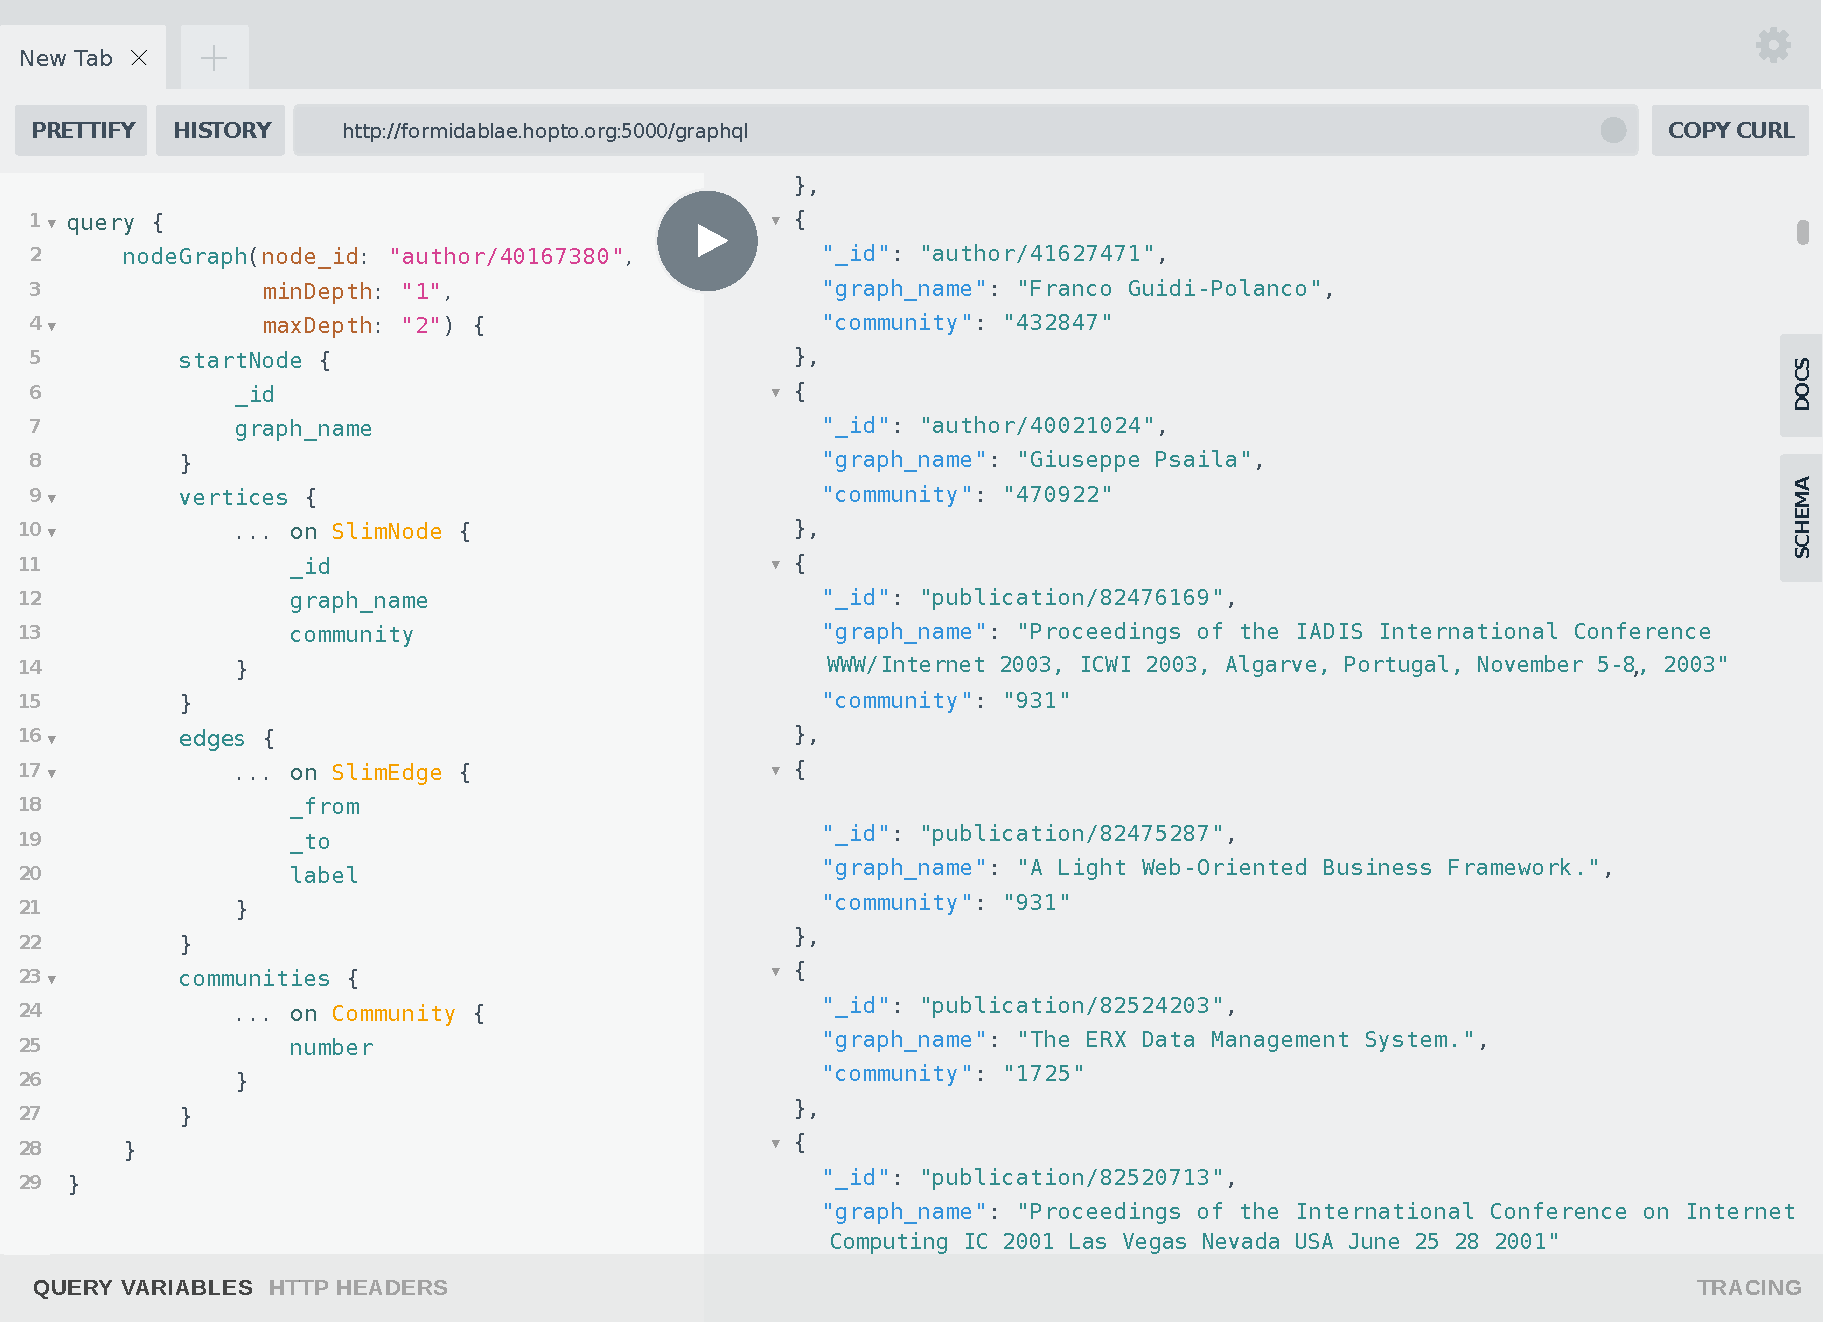
\includegraphics[%
			width=1\textwidth-4pt,%
			bgcolor=white,%
			cfbox=lightestgray % color
				  2pt % rule width
				  0pt % rule separation
				  0pt % margin
		]{images/appendixB/PlaygroundQueryGraphQLBrugali.pdf}%
		\caption[Example query in GraphQL Playground for graph data retrieval]{Example query in \gls{GraphQL Playground} for graph data retrieval}%
		\label{fig:PlaygroundQueryGraphQLBrugali}%
\end{figure}%

Once the request is sent, the response shown on the right of \hyperref[fig:PlaygroundQueryGraphQLBrugali]{\autoref{fig:PlaygroundQueryGraphQLBrugali}} is obtained.

\newpage
\thispagestyle{empty}
